\documentclass[12pt]{article}

\usepackage[margin=1in]{geometry}
\usepackage[version=3]{mhchem}
\usepackage{graphicx}
\usepackage{subfig}
\usepackage{fancyhdr}
\usepackage{amsmath}
\usepackage{fancyvrb}
\usepackage{color}
\usepackage{multirow}

\makeatletter
\def\PY@reset{\let\PY@it=\relax \let\PY@bf=\relax%
    \let\PY@ul=\relax \let\PY@tc=\relax%
    \let\PY@bc=\relax \let\PY@ff=\relax}
\def\PY@tok#1{\csname PY@tok@#1\endcsname}
\def\PY@toks#1+{\ifx\relax#1\empty\else%
    \PY@tok{#1}\expandafter\PY@toks\fi}
\def\PY@do#1{\PY@bc{\PY@tc{\PY@ul{%
    \PY@it{\PY@bf{\PY@ff{#1}}}}}}}
\def\PY#1#2{\PY@reset\PY@toks#1+\relax+\PY@do{#2}}

\expandafter\def\csname PY@tok@gd\endcsname{\def\PY@tc##1{\textcolor[rgb]{0.63,0.00,0.00}{##1}}}
\expandafter\def\csname PY@tok@gu\endcsname{\let\PY@bf=\textbf\def\PY@tc##1{\textcolor[rgb]{0.50,0.00,0.50}{##1}}}
\expandafter\def\csname PY@tok@gt\endcsname{\def\PY@tc##1{\textcolor[rgb]{0.00,0.27,0.87}{##1}}}
\expandafter\def\csname PY@tok@gs\endcsname{\let\PY@bf=\textbf}
\expandafter\def\csname PY@tok@gr\endcsname{\def\PY@tc##1{\textcolor[rgb]{1.00,0.00,0.00}{##1}}}
\expandafter\def\csname PY@tok@cm\endcsname{\let\PY@it=\textit\def\PY@tc##1{\textcolor[rgb]{0.25,0.50,0.50}{##1}}}
\expandafter\def\csname PY@tok@vg\endcsname{\def\PY@tc##1{\textcolor[rgb]{0.10,0.09,0.49}{##1}}}
\expandafter\def\csname PY@tok@m\endcsname{\def\PY@tc##1{\textcolor[rgb]{0.40,0.40,0.40}{##1}}}
\expandafter\def\csname PY@tok@mh\endcsname{\def\PY@tc##1{\textcolor[rgb]{0.40,0.40,0.40}{##1}}}
\expandafter\def\csname PY@tok@go\endcsname{\def\PY@tc##1{\textcolor[rgb]{0.53,0.53,0.53}{##1}}}
\expandafter\def\csname PY@tok@ge\endcsname{\let\PY@it=\textit}
\expandafter\def\csname PY@tok@vc\endcsname{\def\PY@tc##1{\textcolor[rgb]{0.10,0.09,0.49}{##1}}}
\expandafter\def\csname PY@tok@il\endcsname{\def\PY@tc##1{\textcolor[rgb]{0.40,0.40,0.40}{##1}}}
\expandafter\def\csname PY@tok@cs\endcsname{\let\PY@it=\textit\def\PY@tc##1{\textcolor[rgb]{0.25,0.50,0.50}{##1}}}
\expandafter\def\csname PY@tok@cp\endcsname{\def\PY@tc##1{\textcolor[rgb]{0.74,0.48,0.00}{##1}}}
\expandafter\def\csname PY@tok@gi\endcsname{\def\PY@tc##1{\textcolor[rgb]{0.00,0.63,0.00}{##1}}}
\expandafter\def\csname PY@tok@gh\endcsname{\let\PY@bf=\textbf\def\PY@tc##1{\textcolor[rgb]{0.00,0.00,0.50}{##1}}}
\expandafter\def\csname PY@tok@ni\endcsname{\let\PY@bf=\textbf\def\PY@tc##1{\textcolor[rgb]{0.60,0.60,0.60}{##1}}}
\expandafter\def\csname PY@tok@nl\endcsname{\def\PY@tc##1{\textcolor[rgb]{0.63,0.63,0.00}{##1}}}
\expandafter\def\csname PY@tok@nn\endcsname{\let\PY@bf=\textbf\def\PY@tc##1{\textcolor[rgb]{0.00,0.00,1.00}{##1}}}
\expandafter\def\csname PY@tok@no\endcsname{\def\PY@tc##1{\textcolor[rgb]{0.53,0.00,0.00}{##1}}}
\expandafter\def\csname PY@tok@na\endcsname{\def\PY@tc##1{\textcolor[rgb]{0.49,0.56,0.16}{##1}}}
\expandafter\def\csname PY@tok@nb\endcsname{\def\PY@tc##1{\textcolor[rgb]{0.00,0.50,0.00}{##1}}}
\expandafter\def\csname PY@tok@nc\endcsname{\let\PY@bf=\textbf\def\PY@tc##1{\textcolor[rgb]{0.00,0.00,1.00}{##1}}}
\expandafter\def\csname PY@tok@nd\endcsname{\def\PY@tc##1{\textcolor[rgb]{0.67,0.13,1.00}{##1}}}
\expandafter\def\csname PY@tok@ne\endcsname{\let\PY@bf=\textbf\def\PY@tc##1{\textcolor[rgb]{0.82,0.25,0.23}{##1}}}
\expandafter\def\csname PY@tok@nf\endcsname{\def\PY@tc##1{\textcolor[rgb]{0.00,0.00,1.00}{##1}}}
\expandafter\def\csname PY@tok@si\endcsname{\let\PY@bf=\textbf\def\PY@tc##1{\textcolor[rgb]{0.73,0.40,0.53}{##1}}}
\expandafter\def\csname PY@tok@s2\endcsname{\def\PY@tc##1{\textcolor[rgb]{0.73,0.13,0.13}{##1}}}
\expandafter\def\csname PY@tok@vi\endcsname{\def\PY@tc##1{\textcolor[rgb]{0.10,0.09,0.49}{##1}}}
\expandafter\def\csname PY@tok@nt\endcsname{\let\PY@bf=\textbf\def\PY@tc##1{\textcolor[rgb]{0.00,0.50,0.00}{##1}}}
\expandafter\def\csname PY@tok@nv\endcsname{\def\PY@tc##1{\textcolor[rgb]{0.10,0.09,0.49}{##1}}}
\expandafter\def\csname PY@tok@s1\endcsname{\def\PY@tc##1{\textcolor[rgb]{0.73,0.13,0.13}{##1}}}
\expandafter\def\csname PY@tok@kd\endcsname{\let\PY@bf=\textbf\def\PY@tc##1{\textcolor[rgb]{0.00,0.50,0.00}{##1}}}
\expandafter\def\csname PY@tok@sh\endcsname{\def\PY@tc##1{\textcolor[rgb]{0.73,0.13,0.13}{##1}}}
\expandafter\def\csname PY@tok@sc\endcsname{\def\PY@tc##1{\textcolor[rgb]{0.73,0.13,0.13}{##1}}}
\expandafter\def\csname PY@tok@sx\endcsname{\def\PY@tc##1{\textcolor[rgb]{0.00,0.50,0.00}{##1}}}
\expandafter\def\csname PY@tok@bp\endcsname{\def\PY@tc##1{\textcolor[rgb]{0.00,0.50,0.00}{##1}}}
\expandafter\def\csname PY@tok@c1\endcsname{\let\PY@it=\textit\def\PY@tc##1{\textcolor[rgb]{0.25,0.50,0.50}{##1}}}
\expandafter\def\csname PY@tok@kc\endcsname{\let\PY@bf=\textbf\def\PY@tc##1{\textcolor[rgb]{0.00,0.50,0.00}{##1}}}
\expandafter\def\csname PY@tok@c\endcsname{\let\PY@it=\textit\def\PY@tc##1{\textcolor[rgb]{0.25,0.50,0.50}{##1}}}
\expandafter\def\csname PY@tok@mf\endcsname{\def\PY@tc##1{\textcolor[rgb]{0.40,0.40,0.40}{##1}}}
\expandafter\def\csname PY@tok@err\endcsname{\def\PY@bc##1{\setlength{\fboxsep}{0pt}\fcolorbox[rgb]{1.00,0.00,0.00}{1,1,1}{\strut ##1}}}
\expandafter\def\csname PY@tok@mb\endcsname{\def\PY@tc##1{\textcolor[rgb]{0.40,0.40,0.40}{##1}}}
\expandafter\def\csname PY@tok@ss\endcsname{\def\PY@tc##1{\textcolor[rgb]{0.10,0.09,0.49}{##1}}}
\expandafter\def\csname PY@tok@sr\endcsname{\def\PY@tc##1{\textcolor[rgb]{0.73,0.40,0.53}{##1}}}
\expandafter\def\csname PY@tok@mo\endcsname{\def\PY@tc##1{\textcolor[rgb]{0.40,0.40,0.40}{##1}}}
\expandafter\def\csname PY@tok@kn\endcsname{\let\PY@bf=\textbf\def\PY@tc##1{\textcolor[rgb]{0.00,0.50,0.00}{##1}}}
\expandafter\def\csname PY@tok@mi\endcsname{\def\PY@tc##1{\textcolor[rgb]{0.40,0.40,0.40}{##1}}}
\expandafter\def\csname PY@tok@gp\endcsname{\let\PY@bf=\textbf\def\PY@tc##1{\textcolor[rgb]{0.00,0.00,0.50}{##1}}}
\expandafter\def\csname PY@tok@o\endcsname{\def\PY@tc##1{\textcolor[rgb]{0.40,0.40,0.40}{##1}}}
\expandafter\def\csname PY@tok@kr\endcsname{\let\PY@bf=\textbf\def\PY@tc##1{\textcolor[rgb]{0.00,0.50,0.00}{##1}}}
\expandafter\def\csname PY@tok@s\endcsname{\def\PY@tc##1{\textcolor[rgb]{0.73,0.13,0.13}{##1}}}
\expandafter\def\csname PY@tok@kp\endcsname{\def\PY@tc##1{\textcolor[rgb]{0.00,0.50,0.00}{##1}}}
\expandafter\def\csname PY@tok@w\endcsname{\def\PY@tc##1{\textcolor[rgb]{0.73,0.73,0.73}{##1}}}
\expandafter\def\csname PY@tok@kt\endcsname{\def\PY@tc##1{\textcolor[rgb]{0.69,0.00,0.25}{##1}}}
\expandafter\def\csname PY@tok@ow\endcsname{\let\PY@bf=\textbf\def\PY@tc##1{\textcolor[rgb]{0.67,0.13,1.00}{##1}}}
\expandafter\def\csname PY@tok@sb\endcsname{\def\PY@tc##1{\textcolor[rgb]{0.73,0.13,0.13}{##1}}}
\expandafter\def\csname PY@tok@k\endcsname{\let\PY@bf=\textbf\def\PY@tc##1{\textcolor[rgb]{0.00,0.50,0.00}{##1}}}
\expandafter\def\csname PY@tok@se\endcsname{\let\PY@bf=\textbf\def\PY@tc##1{\textcolor[rgb]{0.73,0.40,0.13}{##1}}}
\expandafter\def\csname PY@tok@sd\endcsname{\let\PY@it=\textit\def\PY@tc##1{\textcolor[rgb]{0.73,0.13,0.13}{##1}}}

\def\PYZbs{\char`\\}
\def\PYZus{\char`\_}
\def\PYZob{\char`\{}
\def\PYZcb{\char`\}}
\def\PYZca{\char`\^}
\def\PYZam{\char`\&}
\def\PYZlt{\char`\<}
\def\PYZgt{\char`\>}
\def\PYZsh{\char`\#}
\def\PYZpc{\char`\%}
\def\PYZdl{\char`\$}
\def\PYZhy{\char`\-}
\def\PYZsq{\char`\'}
\def\PYZdq{\char`\"}
\def\PYZti{\char`\~}
% for compatibility with earlier versions
\def\PYZat{@}
\def\PYZlb{[}
\def\PYZrb{]}
\makeatother


\newcommand{\unit}[1]{\ensuremath{\, \mathrm{#1}}}
\newcommand{\e}[1]{\ensuremath{\times 10^{#1}}}

\pagestyle{fancy}
\lhead{NANO 266 - Quantum Mechanical Modeling}
\rhead{Spring 2015}

\title{NANO 266 - Lab 3}
\author{Zhi Deng \\ PID:A53058446}
\date{May 20, 2015}

\begin{document}

\maketitle
\thispagestyle{fancy}


\clearpage
\section*{Q1}

First of all, perform the $k$-point convergence test on both bcc and hcp Fe with convergence criteria set to 1\unit{meV/atom}.

\begin{itemize}
	\item For bcc Fe, set the lattice parameter $a = 5.42\unit{a.u.}$ Use a $k\times k\times k$ $k$-point grid, where $k$ increases from 8 to 20 with increment 1.
	\item For hcp Fe, set the lattice parameters $a = 4.8\unit{a.u.}$ and $c/a = 1.73$. Use a $k_1\times k_1\times k_3$ $k$-point grid, where $k_1$ increases from 8 to 20 with increment 1, $k_3$ is automatically determined by $k_1$ and $c/a$. For more details on $k_3$, please see the following program and table. 
\end{itemize}

\begin{Verbatim}[commandchars=\\\{\},frame=single]
\PY{k+kn}{import} \PY{n+nn}{numpy} \PY{k+kn}{as} \PY{n+nn}{np}
\PY{n}{calat} \PY{o}{=} \PY{l+m+mf}{1.73}
\PY{n}{k1\PYZus{}array} \PY{o}{=} \PY{n}{np}\PY{o}{.}\PY{n}{arange}\PY{p}{(}\PY{l+m+mi}{8}\PY{p}{,}\PY{l+m+mi}{21}\PY{p}{)}
\PY{n}{k3\PYZus{}array} \PY{o}{=} \PY{n}{np}\PY{o}{.}\PY{n}{ceil}\PY{p}{(}\PY{n}{k1\PYZus{}array}\PY{o}{/}\PY{n}{calat}\PY{p}{)}\PY{o}{.}\PY{n}{astype}\PY{p}{(}\PY{n+nb}{int}\PY{p}{)}
\end{Verbatim}

\begin{center}
	\begin{tabular}{*{14}{|c}|}
		\hline
		$k_1$ & 8 & 9 & 10 & 11 & 12 & 13 & 14 & 15 & 16 & 17 & 18 & 19 & 20 \\
		\hline
		$k_3$ & 5 & 6 & 6 & 7 & 7 & 8 & 9 & 9 & 10 & 10 & 11 & 11 & 12 \\
		\hline
	\end{tabular}
\end{center}

Convergence test results:
\begin{itemize}
	\item bcc Fe converges at $15\times15\times15$ $k$-point grid.
	\item fcc Fe converges at $16\times16\times10$ $k$-point grid.
\end{itemize}

Use the converged $k$-mesh for the following calculations. 

\begin{figure}[h]
\begin{center}
	\subfloat[bcc Fe]{
		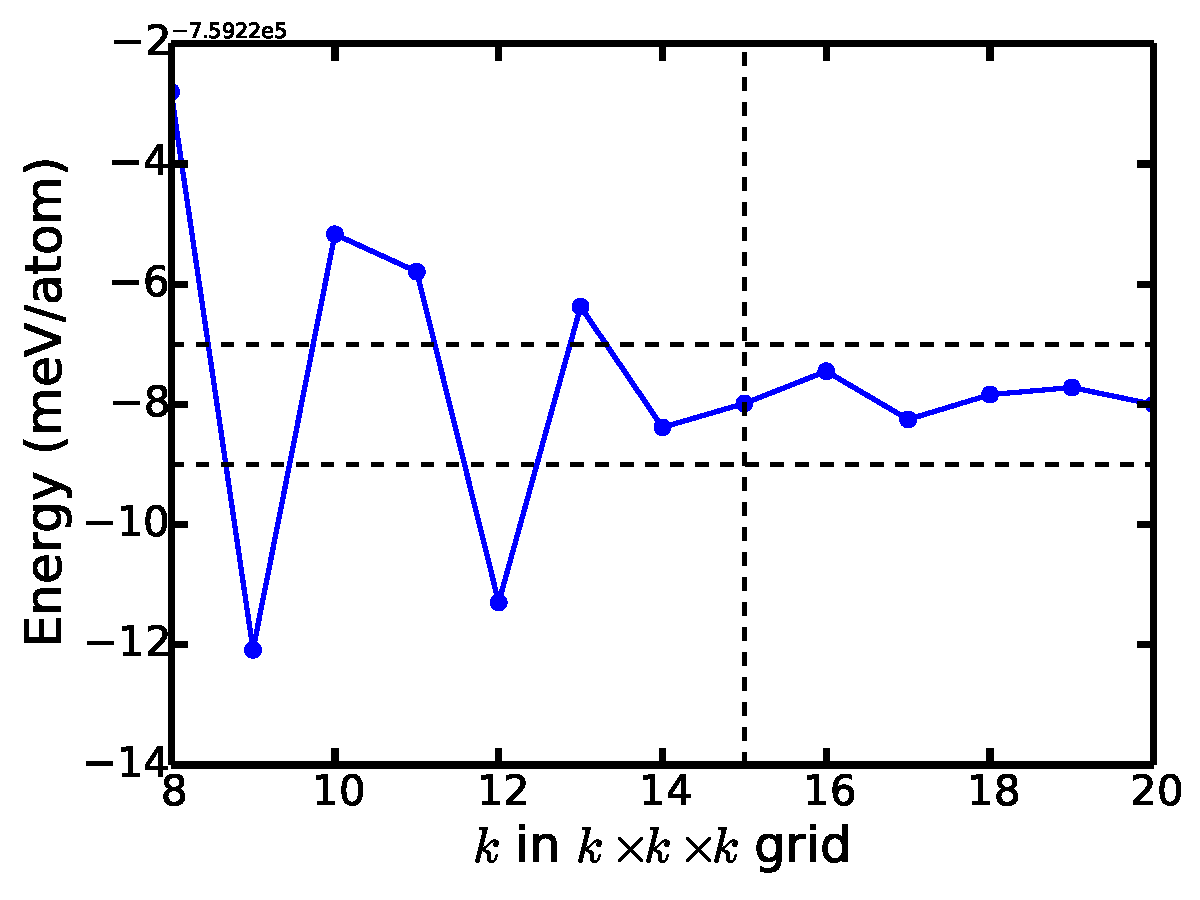
\includegraphics[width=0.45\textwidth]{bcc_kpts}
	}
	\quad
	\subfloat[hcp Fe]{
		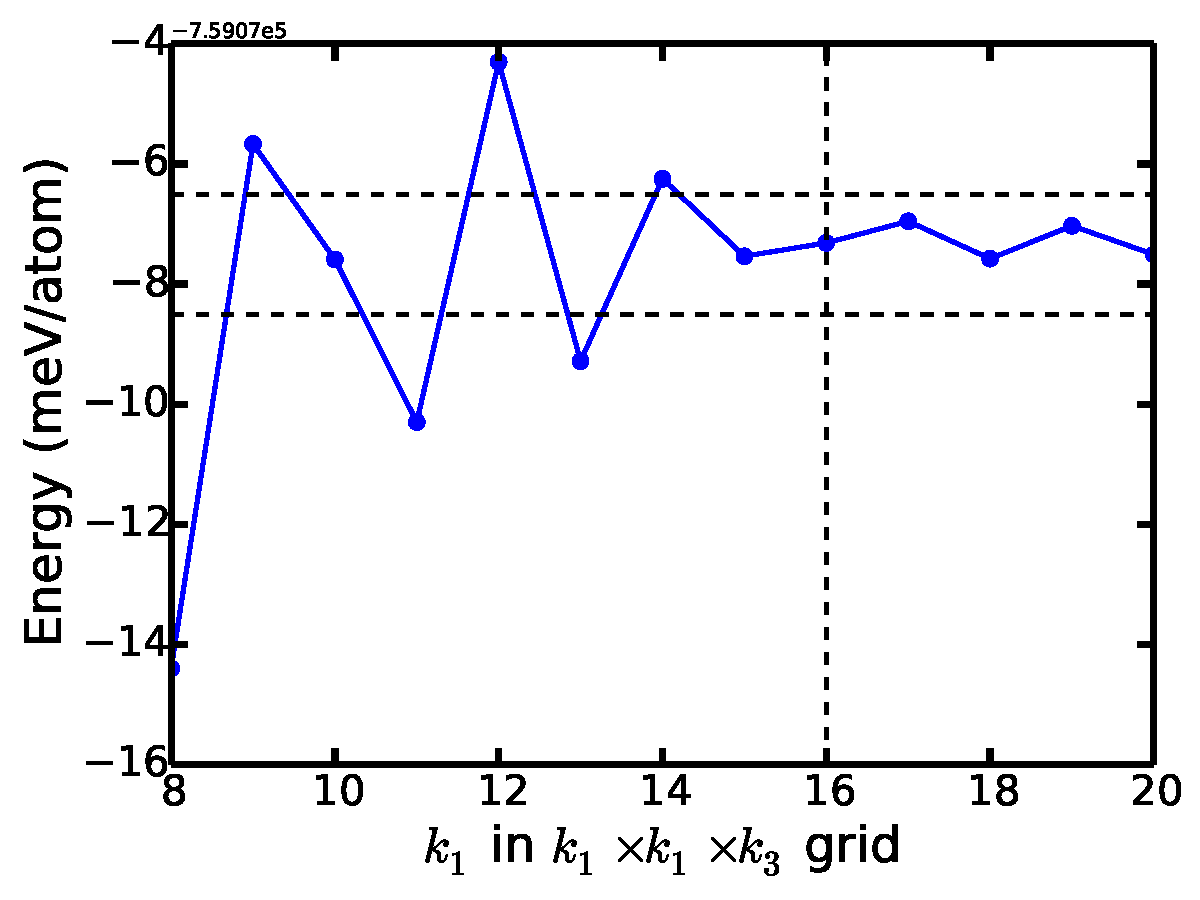
\includegraphics[width=0.45\textwidth]{hcp_kpts}
	}
\end{center}
\end{figure}

\subsection*{1}

Calculate and plot the ground state energy of bcc and hcp Fe near the equilibrium lattice constant. For bcc Fe, the equilibrium lattice constant $a_0 = 2.842\unit{\AA} = 5.37\unit{a.u.}$ For hcp Fe, the equilibrium lattice constant $a_0 = 2.540\unit{\AA} = 4.80\unit{a.u.}$, and $c/a=1.73$. Note the energy differences between different ratios are small near $a_0$.

\begin{figure}[h]
\begin{center}
	\subfloat[bcc Fe]{
		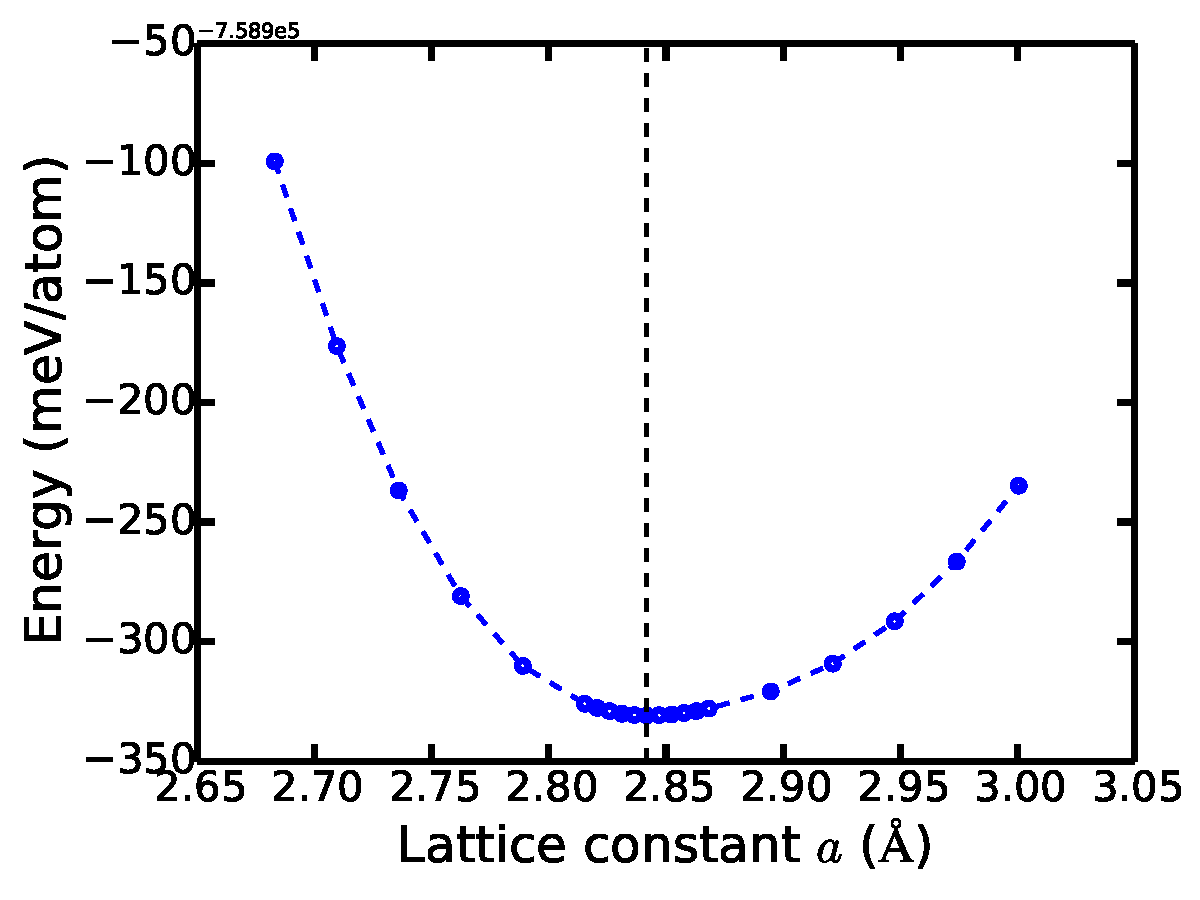
\includegraphics[width=0.5\textwidth]{bcc_latt}
	}
	\subfloat[hcp Fe]{
		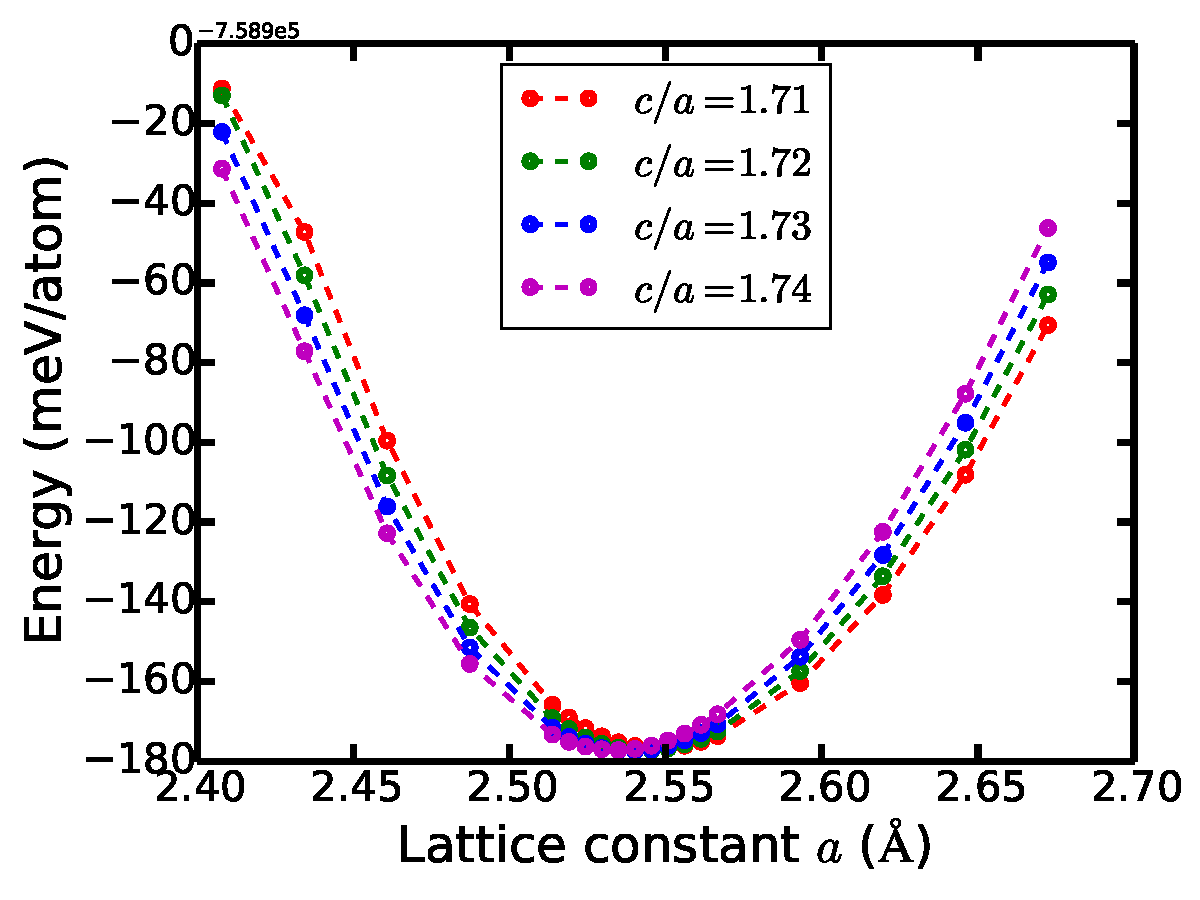
\includegraphics[width=0.5\textwidth]{hcp_latt}
	}
\end{center}
\end{figure}

\subsection*{2}

In thermodynamics, pressure is defined as: 
\begin{flalign*}
	p = -\frac{\partial U}{\partial V},
\end{flalign*}
where $U$ is the internal energy and $V$ is the volume. The internal energy is the total energy from DFT calculation. On the $E$-$V$ plot, the pressure on certain point can be calculated from the slope of the tangent line at that point. 

The Gibbs free energy change is given by
\begin{flalign*}
	\Delta G = \Delta U + p\Delta V - T\Delta S, 
\end{flalign*}
where $T$ is the temperature, $\Delta S$ is the entropy change. The contribution of entropy is relatively small comparing with the other terms in solids. Therefore, 
\begin{flalign*}
	\Delta G = \Delta U + p\Delta V.
\end{flalign*}
The phase transition occurs when the 2 phases have the same Gibbs free energy ($\Delta G=0$). Even with a difference in internal (total) energy, 2 structures can have the same Gibbs free energy as long as they satisfy the following condition: 
\begin{flalign*}
	\Delta U = -p\Delta V.
\end{flalign*}
For this case, on the $E$-$V$ plot, the 2 points on different curves share a common tangent line as the phase transition pressure is unique. 

The cell volume can be calculated from lattice parameters with the following equations:
\begin{flalign*}
	V_{\rm bcc} = a^3, V_{\rm hcp} = \frac{\sqrt{3}}{2}\left(\frac{c}{a}\right)a^3 
\end{flalign*}

Plot the energy of bcc and hcp Fe against cell volume. For the hcp structure, the choice of $c/a$ has no effect on the $E$-$V$ curve. All the curves from different $c/a$ will merge into one curve on the $E$-$V$ plot. (tested)

To find the common tangent line, first fit each curve to a 4-degree polynomial
\begin{flalign*}
	y(x) = ax^4 + bx^3 + cx^2 + dx + e, 
\end{flalign*}
The derivative of the above function is given by: 
\begin{flalign*}
	y'(x) = 4ax^3 + 3bx^2 + 2cx +d. 
\end{flalign*}
The equation of the tangent line passing through an arbitrary point $(x_0,y(x_0))$ on the curve is given by:
\begin{flalign*}
	&y - y(x_0) = y'(x_0)(x - x_0)  \\
	&y = y'(x_0)x - y'(x_0)x_0 + y(x_0)
\end{flalign*}
The common tangent line passing through 2 points of tangency $(x_1,y_1(x_1))$ and $(x_2,y_2(x_2))$ on different curves should have the same slope and intercept. Therefore, 
\begin{flalign*}
	\begin{cases}
		y_1'(x_1) = y_2'(x_2) \\
		- y_1'(x_1)x_1 + y_1(x_1) = - y_2'(x_2)x_2 + y_2(x_2)
	\end{cases}
\end{flalign*}
Solve the equations to get the coordinates of the 2 points of tangency to get the common tangent line. 

Thanks to NumPy and SciPy, I was able to solve them numerically without even knowing the equation of either curve. The source code is available at: %\\https://github.com/adengz/nano266/blob/master/labs/lab3/pressure.py

\clearpage

\begin{figure}[h]
\begin{center}
	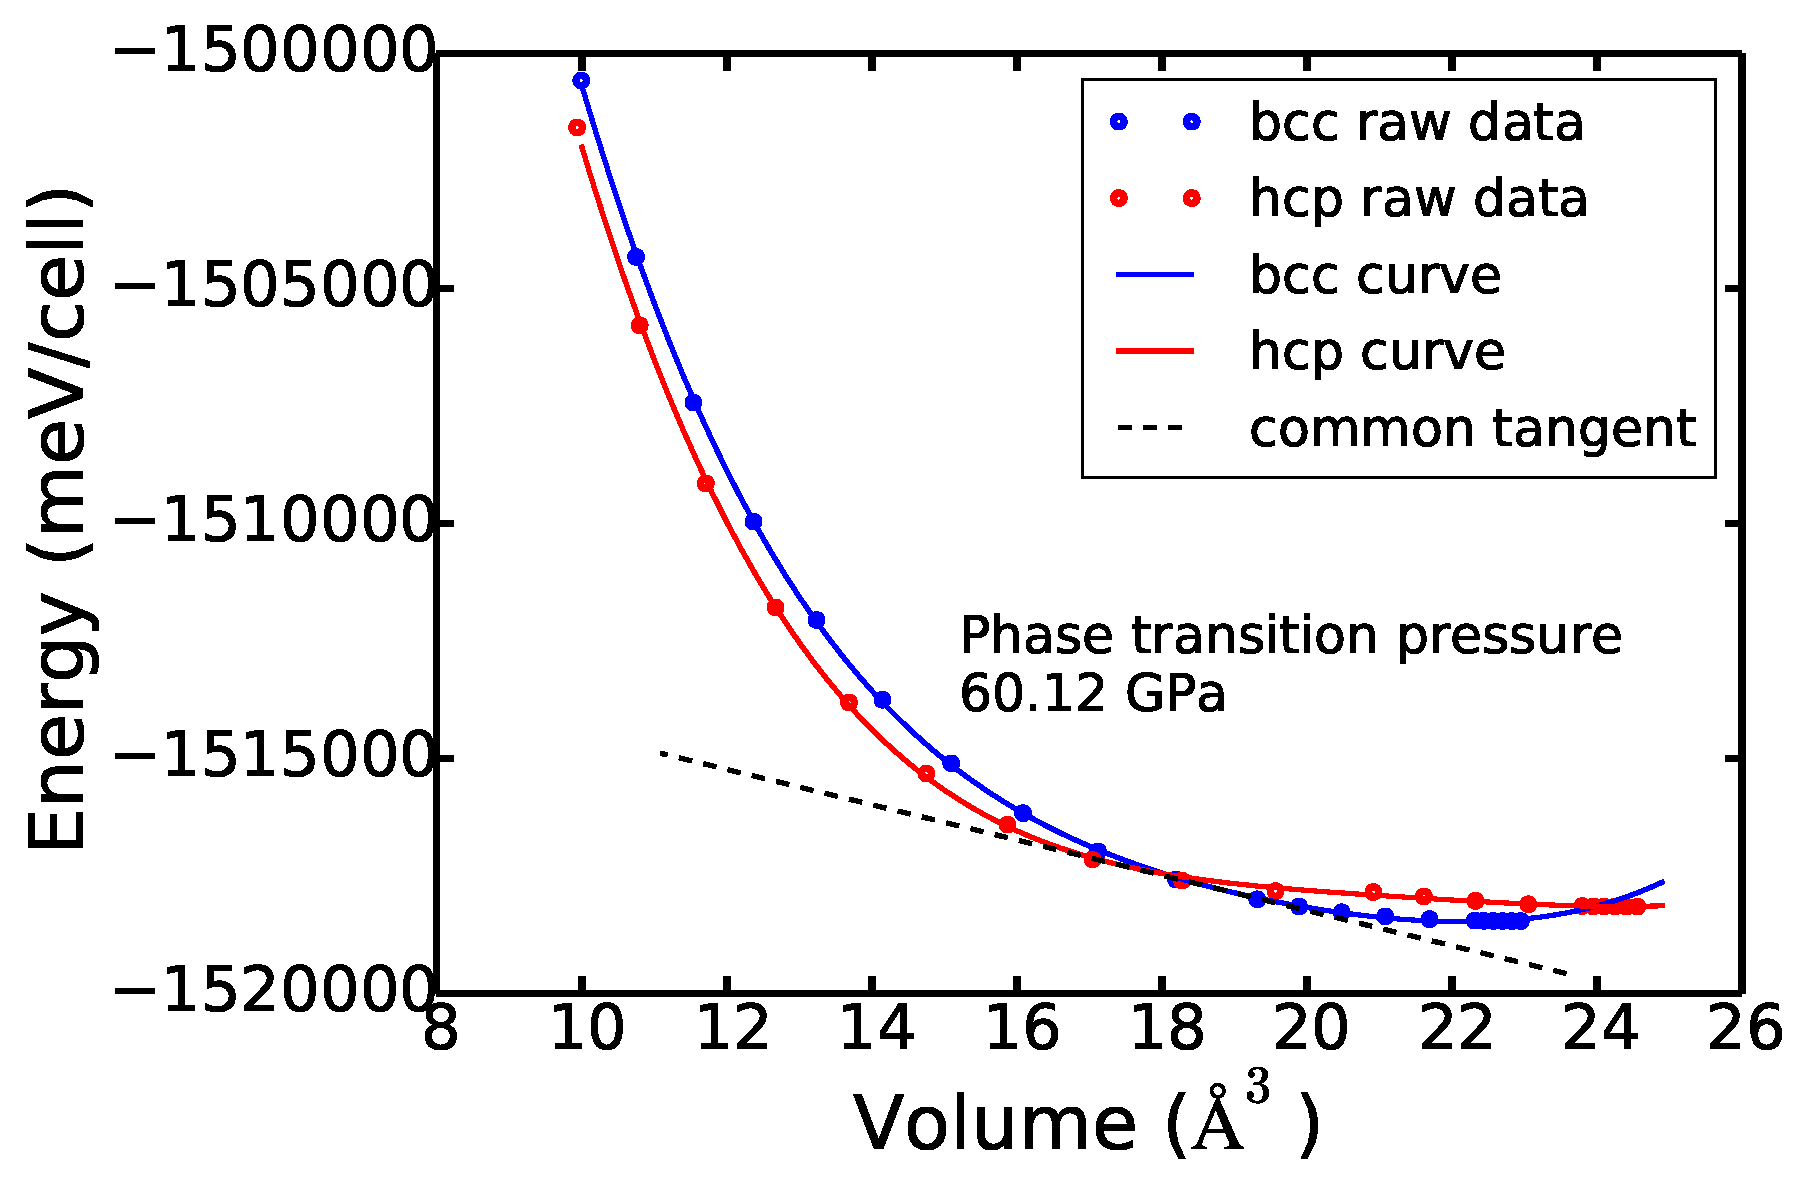
\includegraphics[width=.8\textwidth]{press}
\end{center}
\end{figure}

With the data of 2 tangent points, the pressure is calculated as:
\begin{flalign*}
	p = -\frac{\Delta E}{\Delta V} = 60.12\unit{GPa}
\end{flalign*}

\subsection*{3}

To calculate the total energy of bcc Fe in anti-ferromagnetic state, break the bcc symmetry to simple cubic cell with the 2 atoms having the opposite starting magnetization values (2 different species). Do a $k$-point convergence test using the lowest energy structure from ferromagnetic bcc Fe to get the converged total energy. The template is available at:\\https://github.com/adengz/nano266/blob/master/labs/lab3/Fe.sc.pw.in.template

\clearpage
The result shows that the total energy converges at at $10\times10\times10$ $k$-point grid. 

\begin{figure}[h]
\begin{center}
	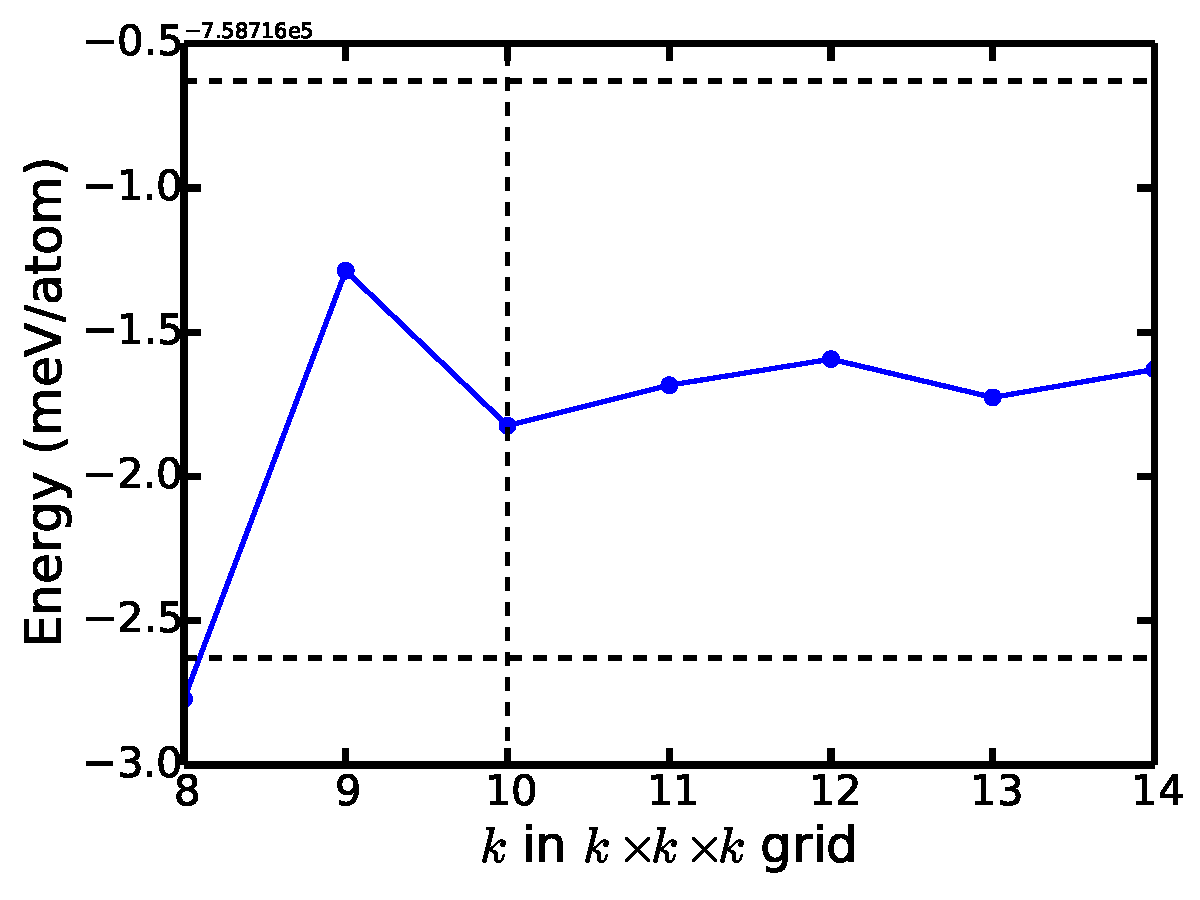
\includegraphics[width=.5\textwidth]{bcc_af_kpts}
\end{center}
\end{figure}

Compare the total energies between ferromagnetic and anti-ferromagnetic states using the converged total energies. The total energy of bcc Fe in ferromagnetic state is around 0.5\unit{eV/atom} lower than that in anti-ferromagnetic state. 

\clearpage
\section*{Q2}

\subsection*{1}

Calculate and plot the energy of cubic \ce{PbTiO3} as a function of lattice parameter. 

\begin{figure}[h]
\begin{center}
	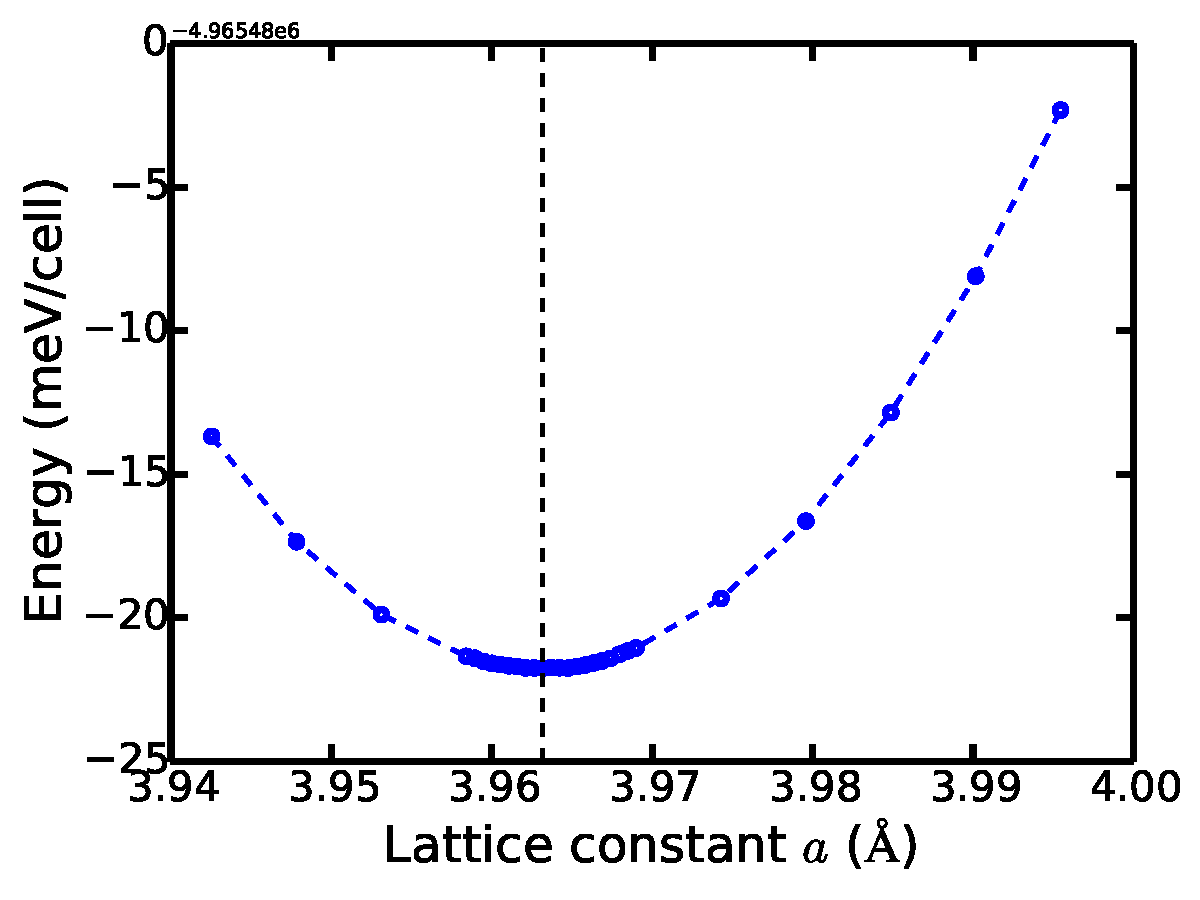
\includegraphics[width=.6\textwidth]{pto_latt}
\end{center}
\end{figure}

At equilibrium, the lattice parameter $a = 3.9632\unit{\AA} = 7.489\unit{a.u.}$

\subsection*{2}

Using the lattice constant at equilibrium, calculate and plot the energy as a function of the displacement of Ti along $c$-axis. 

\begin{figure}[h]
\begin{center}
	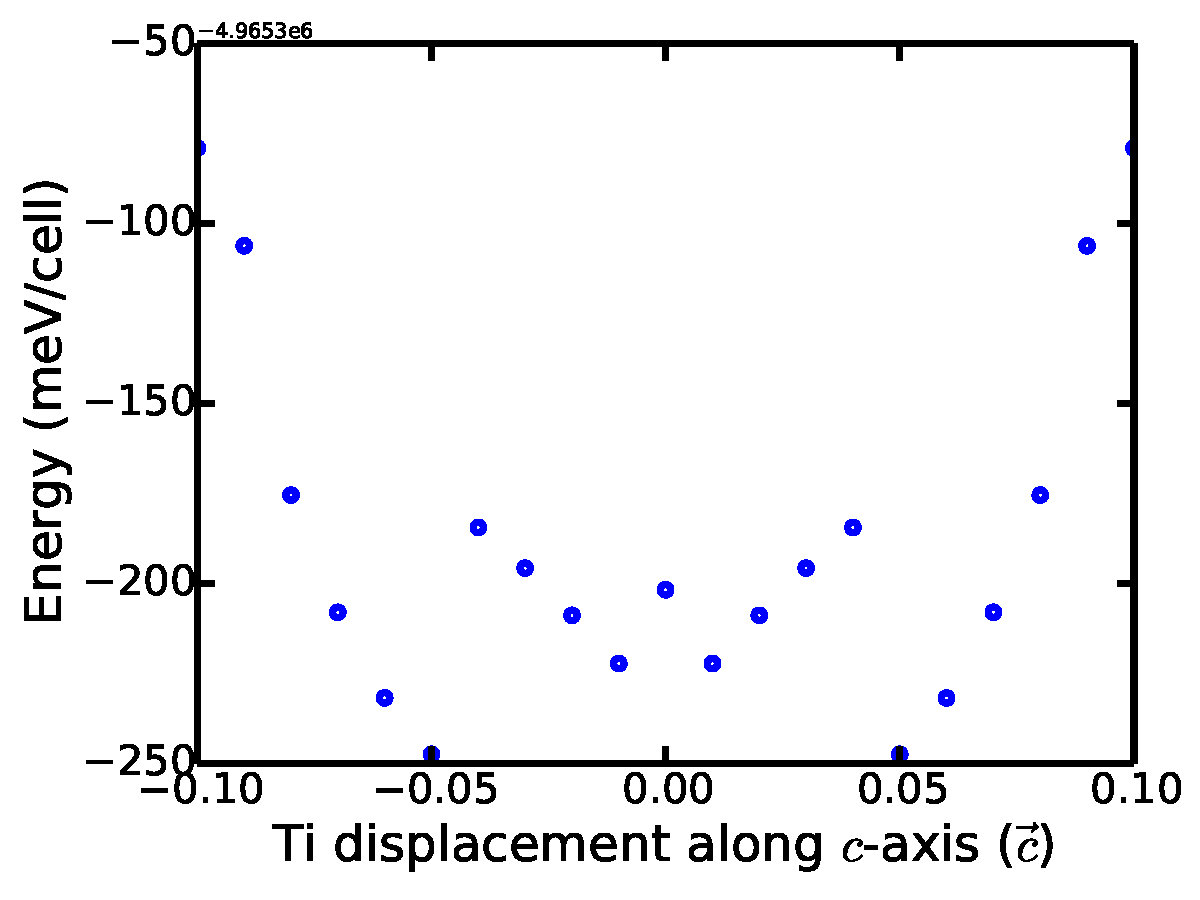
\includegraphics[width=.6\textwidth]{pto_disp}
\end{center}
\end{figure}

The total energy reaches minimum when the displacement of Ti is $\pm0.05\vec{c}$. The energy difference between this configuration and the minimum-energy configuration from previous part is 45.71\unit{meV/fu}. 

\subsection*{3}

Perform the relaxation allowing Ti movement together with O using the configuration with Ti displacement of $0.05\vec{c}$. 

 The final atomic positions are listed in the following table. 
\begin{center}
	\begin{tabular}{|c|c|c|c|}
		\hline
		 & $x$ & $y$ & $z$ \\ \hline
		Pb & 0 & 0 & 0 \\ \hline
		Ti & 0.5 & 0.5 & 0.504526412 \\ \hline
		O & 0.5 & 0.5 & -0.000608651 \\ \hline
		O & 0.5 & 0 & 0.500988678 \\ \hline
		O & 0 & 0.5 & 0.500988678 \\ \hline
	\end{tabular}
\end{center}

Record the final energy to compare the energy differences. 

\subsection*{4}

Using the lowest energy configuration obtained from part 1 as reference, plot the energy difference of the following \ce{PbTiO3} configurations: 
\begin{enumerate}
	\item Ti at (0.5,0.5,0.5). Space group: $Pm\bar{3}m$
	\item Ti at (0.5,0.5,0.55). Space group: $P4mm$
	\item Ti at (0.5,0.5,0.504). Space group: $P4mm$
\end{enumerate}

\begin{figure}[h]
\begin{center}
	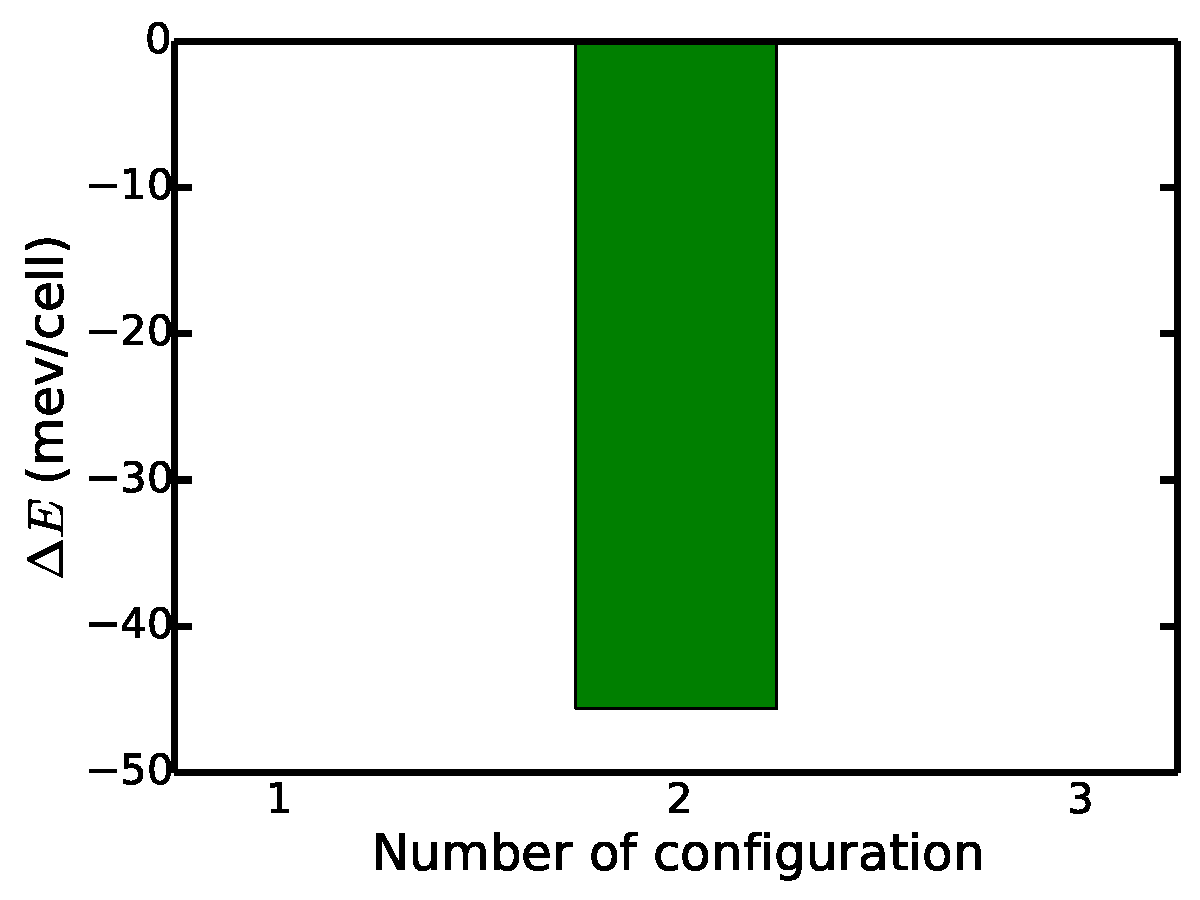
\includegraphics[width=.5\textwidth]{pto_ed}
\end{center}
\end{figure}

The most stable structure is the one with Ti coordinates of (0.5,0.5,0.55). (For the 3rd configuration, I believe the total energy converged to a local minimum)

In the lowest energy structure, the center of mass of positive charges (\ce{Pb^{2+}}) does not coincide with the one of negative charges (\ce{TiO4} tetrahedra). The non-polarized structure (with space group $Pm\bar{3}m$) tends to polarize due to the energy difference, which explains the spontaneous electric polarization, i.e., the ferroelectricity of \ce{PbTiO3}. 


\clearpage
\section*{Q3}

\subsection*{1}

Calculate the ground state energy of Cu, Au and CuAu. The initial guess of lattice constants are listed in the following table. 

\begin{center}
	\begin{tabular}{|c|c|c|}
		\hline
		\multirow{2}{*}{Structure} & \multicolumn{2}{|c|}{$a$} \\ \cline{2-3}
		\multirow{2}{*} & unit: \unit{\AA} & unit: \unit{a.u.} \\ \hline
		fcc Cu & 3.61505 & 6.83 \\ \hline
		fcc Au & 4.17010 & 7.88 \\ \hline
		L$1_0$ CuAu & 3.96900 & 7.50 \\ \hline
	\end{tabular}
\end{center}

Perform the $k$-point convergence test for all structures to get converged total energies. 

\begin{figure}[h]
\begin{center}
	\subfloat[Cu]{
		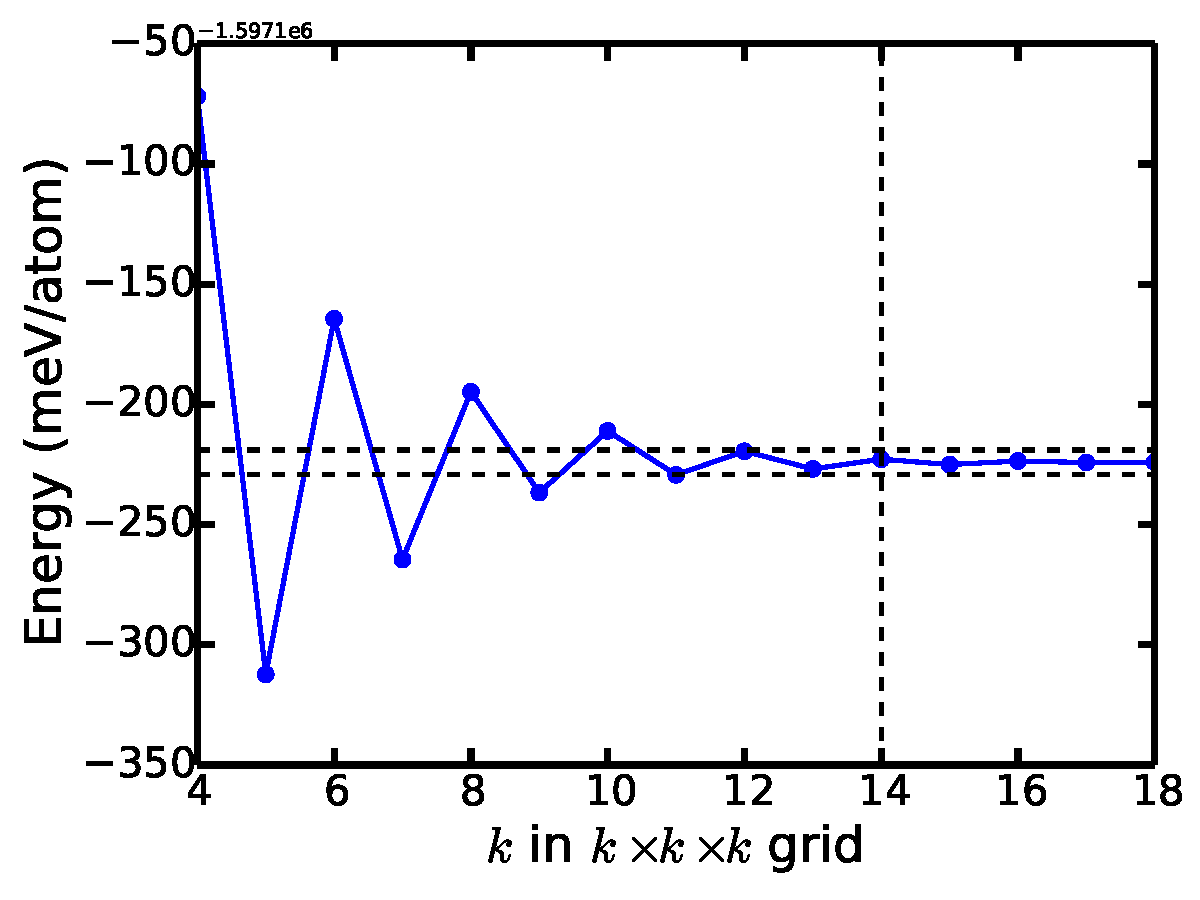
\includegraphics[width=0.45\textwidth]{Cu_kpts}
	}
	\subfloat[Au]{
		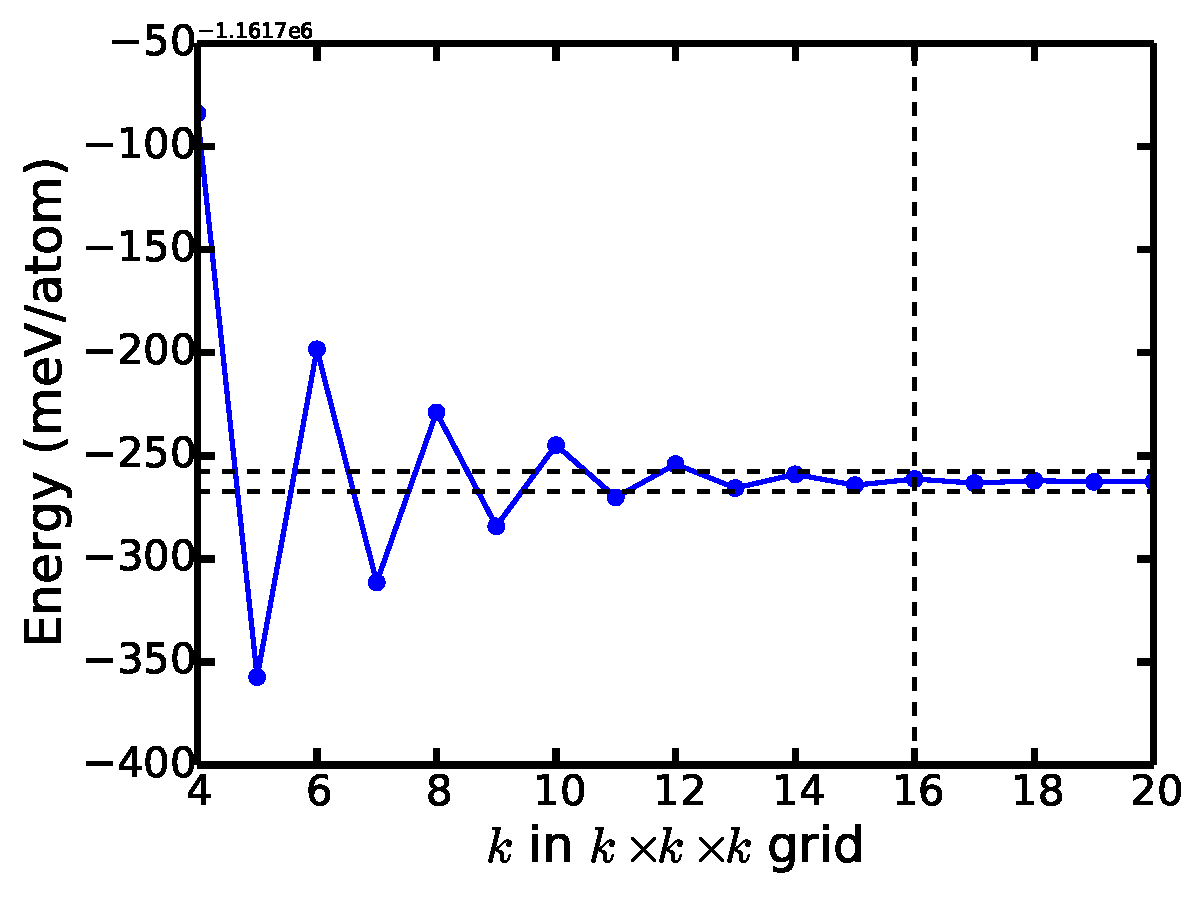
\includegraphics[width=0.45\textwidth]{Au_kpts}
	}\quad
	\subfloat[CuAu]{
		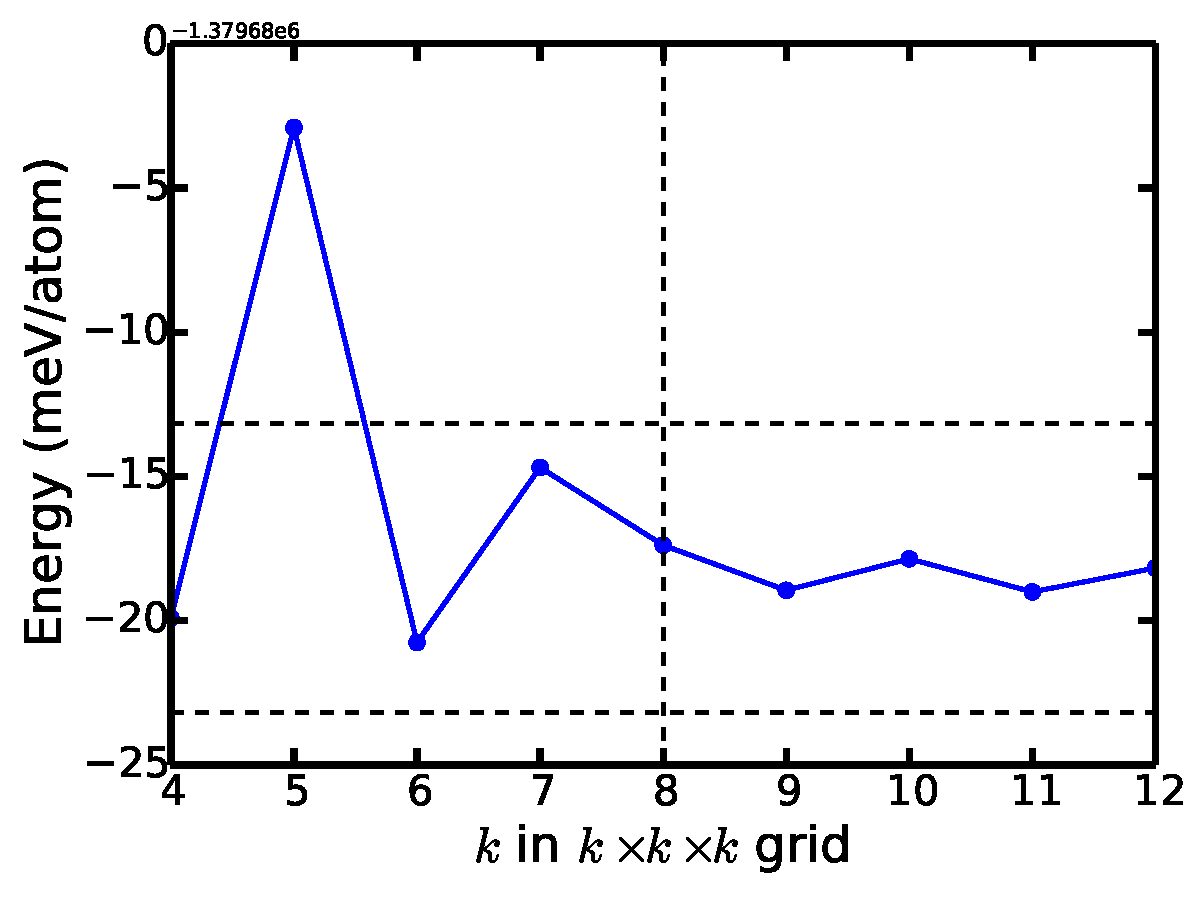
\includegraphics[width=0.45\textwidth]{Cu2Au2_kpts}
	}
\end{center}
\end{figure}

Convergence test results:
\begin{itemize}
	\item Cu converges at $14\times14\times14$ $k$-point grid. The lattice constant $a = 6.88\unit{a.u.}$ for the relaxed structure. 
	\item Au converges at $16\times16\times16$ $k$-point grid. The lattice constant $a = 7.88\unit{a.u.}$ for the relaxed structure. 
	\item CuAu converges at $8\times8\times8$ $k$-point grid.
\end{itemize}

Use the converged total energies for formation energy calculations. 

\subsection*{2}

Calculate the formation energy of \ce{CuAu}. 

\begin{flalign*}
	\Delta H_{\rm f}(\ce{Cu_{0.5}Au_{0.5}}) &= E(\ce{Cu_{0.5}Au_{0.5}}) - 0.5E(\ce{Cu}) - 0.5E(\ce{Au}) & \\
	&= -54.97 \unit{meV/atom} &
\end{flalign*}

\subsection*{3}

Calculate the ground state energy of \ce{Cu3Au} and \ce{CuAu3}. The initial guess on lattice constants are predicted from the relaxed structure of fcc Cu and Au based on Vegard's law ($7.13\unit{a.u.}$ for \ce{Cu3Au} and $7.63\unit{a.u.}$ for \ce{CuAu3}). The $k$-mesh choice should be similar to CuAu as all of them start from simple cubic structure with 4 atoms in the unit cell. 

\begin{figure}[h]
\begin{center}
	\subfloat[\ce{Cu3Au}]{
		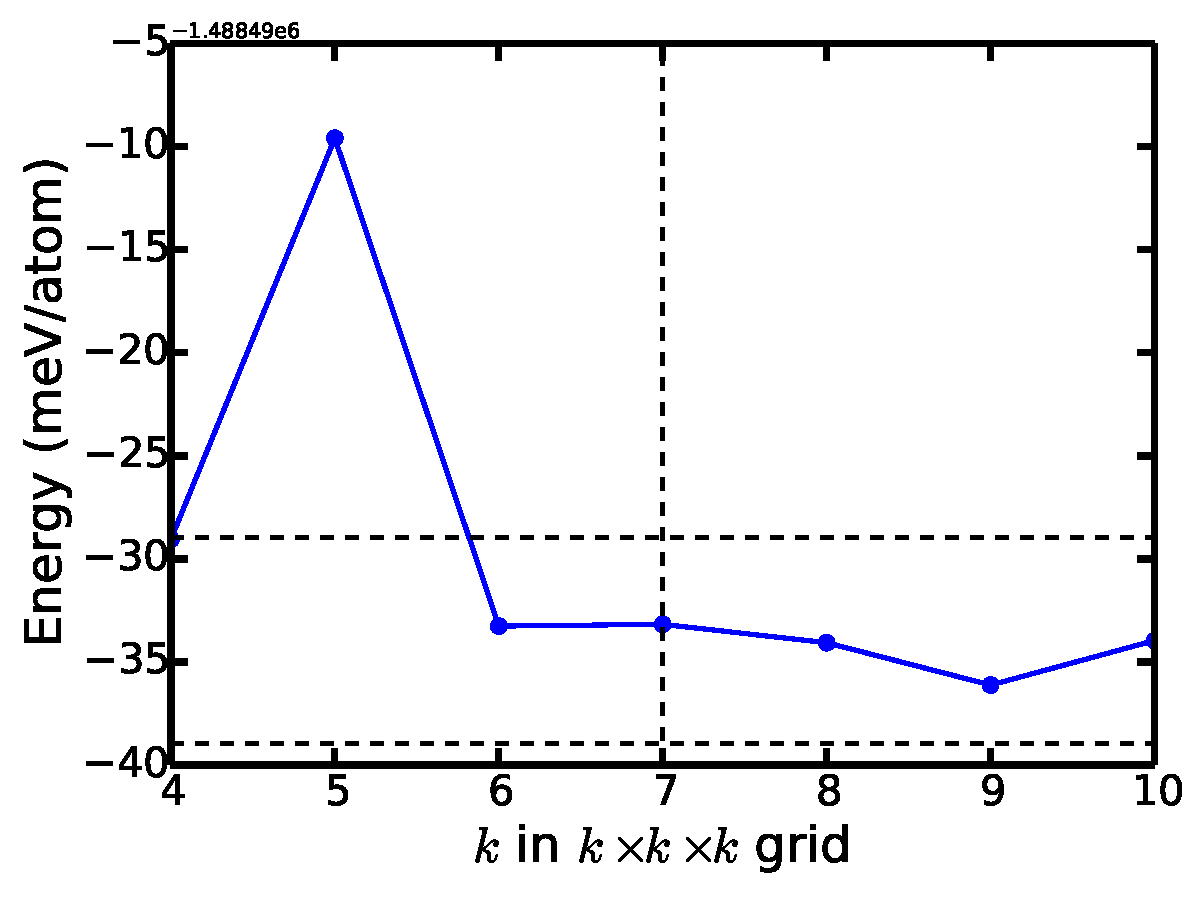
\includegraphics[width=0.45\textwidth]{Cu3Au_kpts}
	}
	\quad
	\subfloat[\ce{CuAu3}]{
		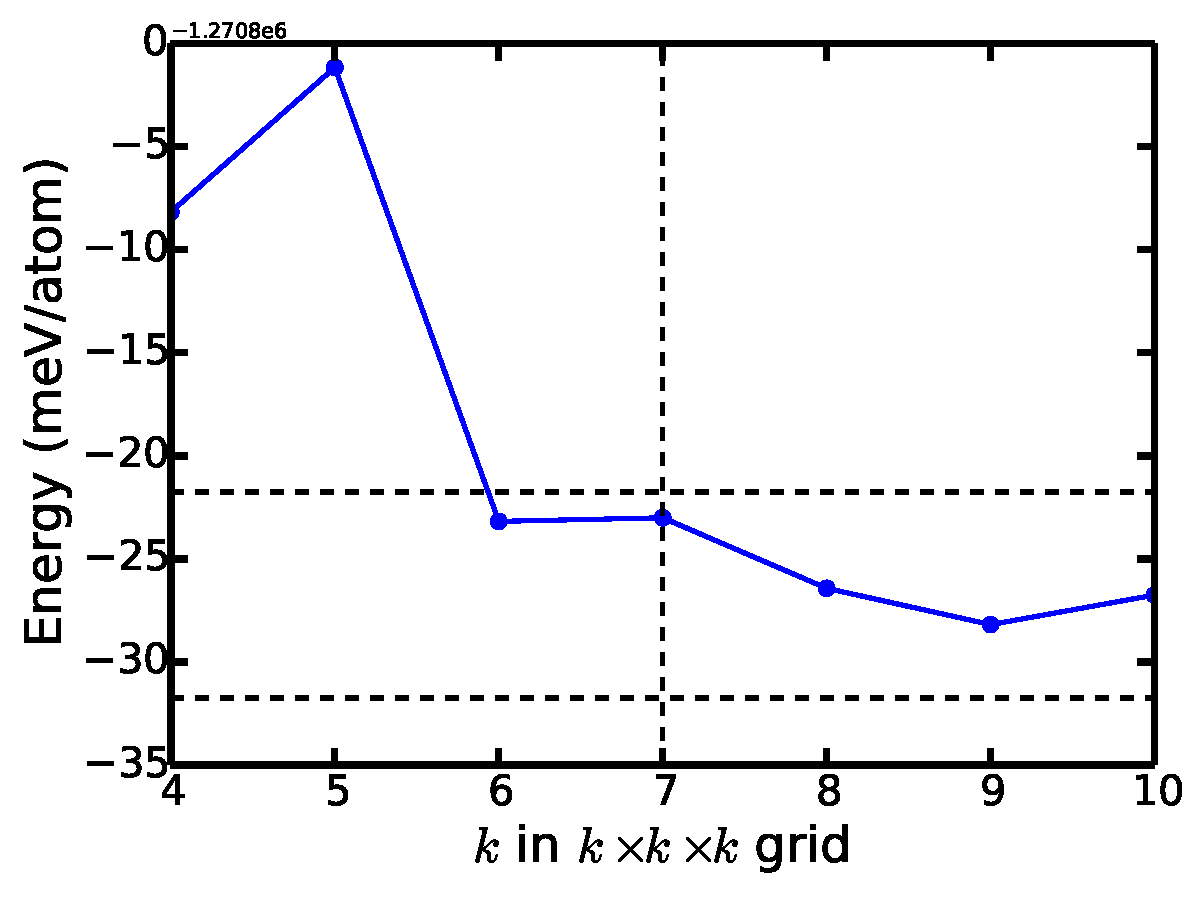
\includegraphics[width=0.45\textwidth]{CuAu3_kpts}
	}
\end{center}
\end{figure}

Both \ce{Cu3Au} and \ce{CuAu3} converges at $7\times7\times7$ $k$-point grid. Use the converged total energies for formation energy calculations. 

\subsection*{4}

Calculate the formation energy of \ce{Cu3Au} and \ce{CuAu3}. 

\begin{flalign*}
	\Delta H_{\rm f}(\ce{Cu_{0.75}Au_{0.25}}) &= E(\ce{Cu_{0.75}Au_{0.25}}) - 0.75E(\ce{Cu}) - 0.25E(\ce{Au}) & \\
	&= -40.35 \unit{meV/atom} & \\
	\Delta H_{\rm f}(\ce{Cu_{0.25}Au_{0.75}}) &= E(\ce{Cu_{0.25}Au_{0.75}}) - 0.25E(\ce{Cu}) - 0.75E(\ce{Au}) & \\
	&= -23.95 \unit{meV/atom} &
\end{flalign*}

Plot the formation energy as a function of $x$ in \ce{Cu_$1-x$Au_$x$} using the phase diagram module in Pymatgen. 

\begin{center}
	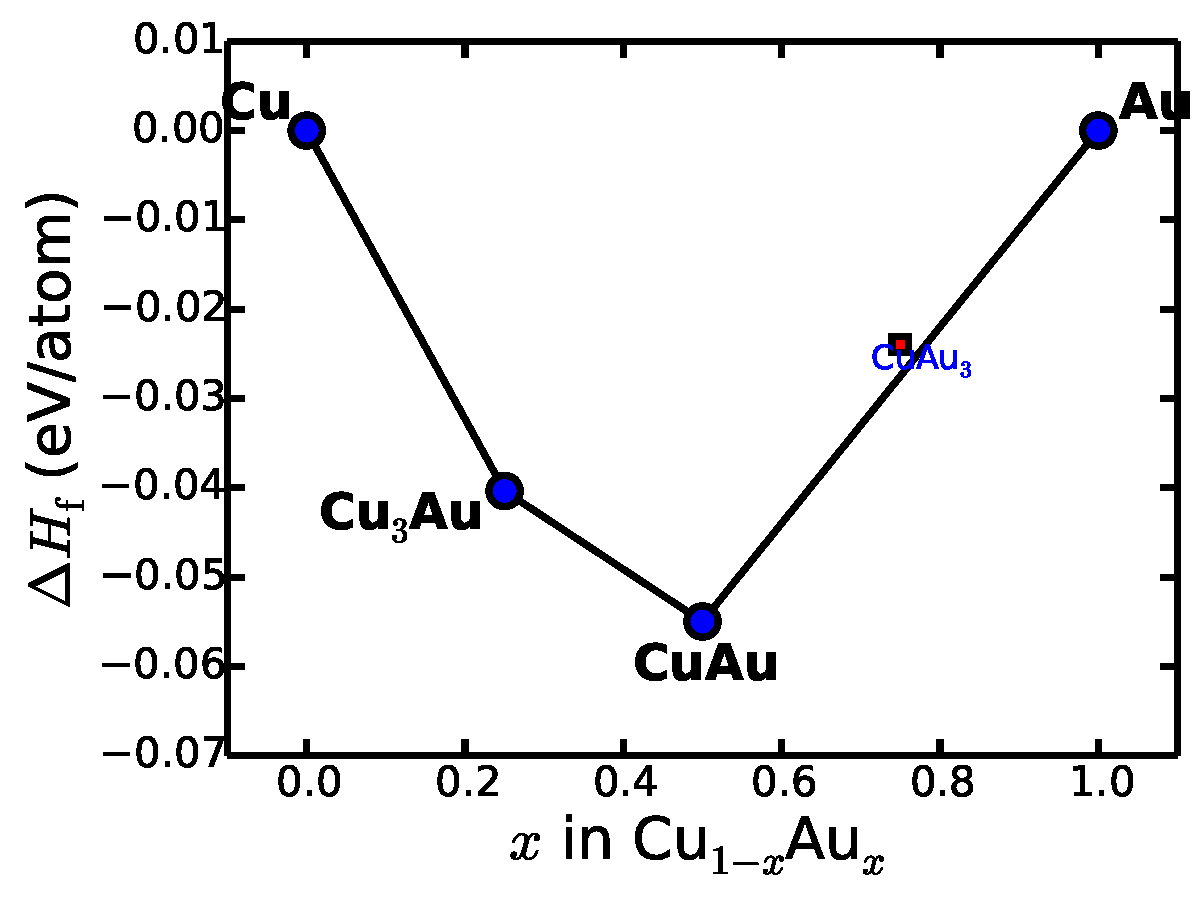
\includegraphics[width=.8\textwidth]{fe}
\end{center}

From the binary phase diagram, we can tell that \ce{Cu3Au} and \ce{CuAu} are stable ordered intermetallic structures at 0\unit{K}. While the formation energy of \ce{CuAu3} is above the convex hull, indicating it's unstable at 0\unit{K}. 

\end{document}